\input{chapter-header.tex}
\newcommand{\VTT}{Mulero\xspace}
\newcommand{\Vtt}{\VTT}
\newcommand{\VT}{\VTT}
\newcommand{\Vt}{\VTT}

% ===========================================================================
\chapter{\VTT: Virtual Language Runtimes}
\minitoc
% ===========================================================================
\introduction
% ===========================================================================

This chapter presents the core contribution of this dissertation: our Virtual Language Runtime infrastructure, namely \VTT~(cf. Section \ref{sec:virtualization_overview}). \VTT allows the monitoring and manipulation of a language runtime through a language hypervisor~(cf. Figure \ref{fig:virtualization_introduction}). In \VTT, both the virtualized runtime and the language hypervisor are first class objects. A first-class representation of a language runtime, namely an \emph{object space}, encapsulates the language runtime and provides a high-level API to query and manipulate it~(cf. Section \ref{sec:object_space}). A first-class \emph{language hypervisor} is a client of an object space~(cf. Section\ref{sec:hypervisor}).

\begin{figure}[htb]
\begin{center}
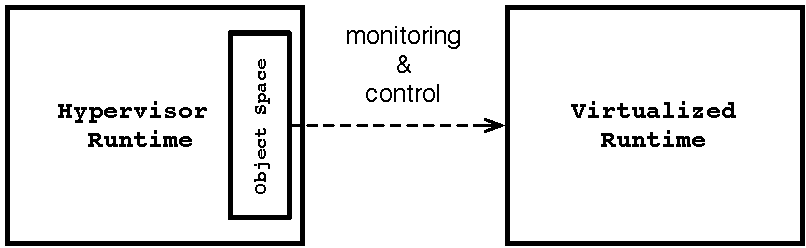
\includegraphics[width=.8\linewidth]{virtualization_introduction}
\caption{\textbf{Virtualization concepts with \Vtt.} A language hypervisor monitors and manipulates a virtualized runtime. Both the virtualized runtime and the language hypervisor share the same process.\label{fig:virtualization_introduction}}
\end{center}
\end{figure}

A language hypervisor runs in the same process than the virtualized runtime to monitor and manipulate it directly. However, the language hypervisor and the virtualized runtime run on different language runtimes: basic objects, classes and VM structures are not shared between the language hypervisor and the virtualized runtime. This has the main purpose of allowing the hypervisor to change any part of the virtualized runtime without affecting itself.

In the rest of this chapter we present in detail these two elements and how they relate to each other. Section \ref{sec:isolation} presents how communication is dealt between an object space and its hypervisor with the no-sharing strategy. Section \ref{sec:execution} explains how we achieve the control of the virtualized runtime through two different strategies: VM execution with safe control points and simulation for a fully managed execution. Finally, Section \ref{sec:virtualization_benchmarks} shows the benchmarks we did on our \Vtt prototype, showing the feasibility of our solution.

%On one side, this means that the hypervisor can freely manipulate the virtualized language runtime without affecting itself. On the other side, this no-sharing strategy poses an extra effort in communication~(cf. Section \emph{sec:isolation}) mainly in object marshaling.

%A language hypervisor is a first-class object in \VTT, meaning that we can easily modify it and replace it by another object. Additionally, a simulation mode allows a fully-managed execution mode.

%We do not require any changes in existing applications to import them inside an object space. We introduce minimal modifications at the \VM level to ensure their control and manipulation is transparent. Regarding execution, an object space provides with different means for controlling the execution of the language runtime it owns~(cf. Section \ref{sec:execution}). It can safely start, pause and resume its execution, create new threads or finalize existing ones.  


\section{\Vtt Architecture} \label{sec:virtualization_overview}

\Vtt presents an architecture where multiple runtime systems can run on the same process independently. They do not share any \VM or language state \ie each one has its own interpreter, stack, classes and objects. A virtualized runtime is a runtime system that is monitored by another runtime system. The runtime system that controls the virtualized runtime is the hypervisor runtime. The hypervisor runtime is a full-fledged object runtime, providing us with the expression power and abstractions of our high level language to express our language hypervisor. To control the virutalized runtime, a hypervisor runtime contains an object space and language hypervisor objects that we use for virtualization purposes. An object space is a first-class object that represents the virtualized runtime and provides operations for its manipulation. A language hypervisor object is the client of such object space implementing a particular manipulation on it \eg runtime update or failure detection.

\begin{figure}[htb]
\begin{center}
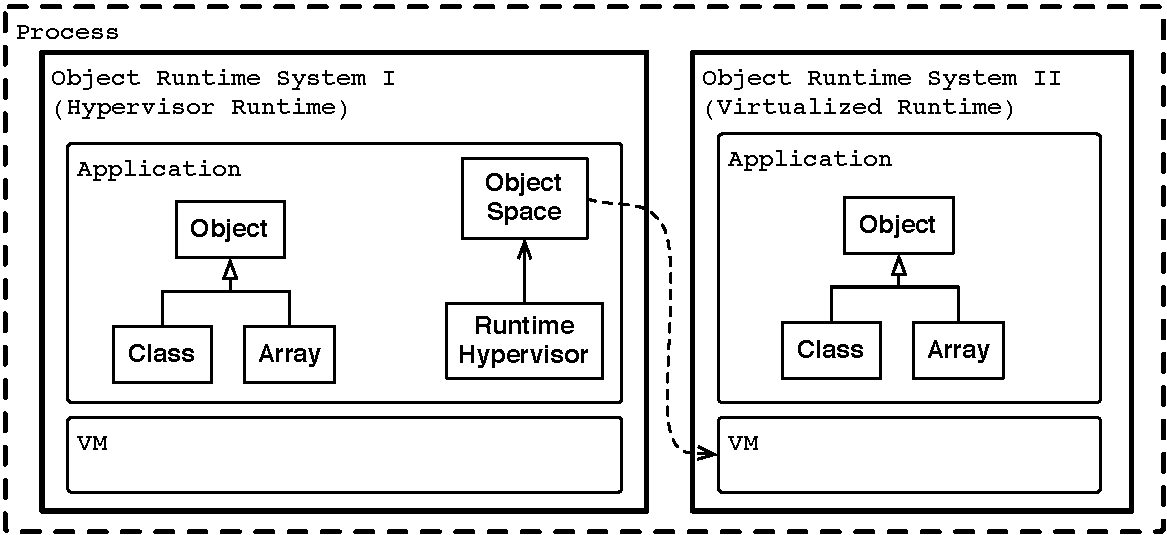
\includegraphics[width=.9\linewidth]{object_space_overview3}
\caption{\textbf{\VTT Overview.} A language hypervisor in the runtime I (left) manipulates the runtime II (right) through an object space. The object space object resides in a different runtime than the one it manipulates.\label{fig:objectSpaceOverview}}
\end{center}
\end{figure}

An object space manipulates the virtualized runtime through directly manipulating the \VM. Doing so at \VM level provides \Vtt with the following properties:

\begin{description}
\item[Transparency.] Our solution does not require any changes in the applications residing inside the virtualized runtime. Thus, we can virtualize existing applications without modifications.
\item[Application independence.] Our solution does not depend on the particular application inside the virtualized runtime. It does depend however on its underlying model imposed by the \VM.
\end{description}

\section{Object Spaces: First-class Language Runtimes} \label{sec:object_space}

An object space is a first-class representation of an object runtime system, meant for its manipulation and control. An object space encapsulates a language runtime and provides with a clear and explicit interface to manipulate it. The object space interface is divided in two different groups of operations: first, operations for the configuration of a VM before it can run; second, operations for the manipulation of the runtime structures at runtime~(objects, classes, threads, the execution stack). This operation is present in two different kind of objects: an \ct{objectSpace} object provides with general operations and mirror objects~\cite{Brac04b} provide with operations to manipulate individual objects.

Object spaces clarify the interface between the language and the VM. On one side, they make explicit what are the elements of the language that should be initialized so the VM can run. On the other side, they also makes explicit which kind of runtime manipulation operations are responsibility of the \VM and which are responsibility of the language.\gp{put an example}

\subsection{VM Setup Interface}

The VM setup is the configuration the VM needs to start running. It is generally composed of the well-known objects of the language such as \ct{nil}, \ct{true} or \ct{false}, special classes that the VM may invoke at runtime, and special messages that the VM will send to the language to notify events ~(\eg the \ct{doesNotUnderstand:} of Smalltalk or \ct{methodMissing} of Ruby). This configuration is usually done only during the language initialisation and not modified afterwards. In particular for bootstrapping, we define the following as the VM setup interface:

\begin{code}
objectSpace\{
    mirror getNil();
    mirror getTrue();
    mirror getFalse();

    void setNil(mirror aNilObject);
    void setTrue(mirror aTrueObject);
    void setFalse(mirror aFalseObject);
    
    mirror getArrayClass();
    void setArrayClass(classMirror anArrayClassMirror);
    ...
    ...
\}
\end{code}

In our particular implementation the list of classes exposed through this interface are those of literal objects and those related with the internal VM execution model. For the sake of completeness the list of classes is the following: \ct{Array}, \ct{Association}, \ct{BlockClosure}, \ct{ByteArray}, \ct{ByteString}, \ct{ByteSymbol}, \ct{Character}, \ct{Context}, \ct{Float}, \ct{SmallInteger}, \ct{LargePositiveInteger}, \ct{LargeNegativeInteger}, \ct{Message}, \ct{CompiledMethod}, \ct{MethodDictionary}, \ct{Semaphore}, \ct{WeakFinalizationList}.

\subsection{Runtime Manipulation Interface} he runtime manipulation interface is composed by operations that the VM uses to manipulate objects at runtime. It contains operations such as reading and writing into a field, set and change and object's class. The bootstrapping interpreter uses this interface to manipulate the objects inside the object space and bootstrap the language kernel. An object space provides also specific kinds of mirrors with higher level APIs to manipulate objects with a specific format and/or behaviour such as classes, methods, activation records or processes. We do not cover these high-level mirrors in this paper as they are not relevant to the bootstrap process.

\begin{code}
objectSpace\{
    mirror createClass(String name, int formatOfInstances);
    mirror getClass(String name);
    void removeClass(String name);
    
    List<mirror> getThreads();
    mirror getContextStackFrame(mirror aThread);
\}

mirror\{
    classMirror getClass().
    void setClass(classMirror aClass).

    mirror getInstanceVariable(String variableName).
    void setInstanceVariable(String variableName, mirror anObject).
    
    void replaceWithObject(mirror object);
\}

classMirror\{
    mirror instantiate();
    mirror instantiate(int aSize);
    
    void compileMethod(String sourceCode);
    void removeMethod(String selector);
\}
\end{code}

Note that from the signatures presented that all mirror operations will return a mirror in exchange. Second, note that a \ct{classMirror} object is also a \ct{mirror} and it shares its operations.
Our object space provides also specific kinds of mirrors with higher level APIs to manipulate objects with a specific format and/or behavior such as classes, methods, activation records or processes. We do not cover these high level mirrors in this paper as they are not relevant to DLU.

% ===========================================================================

\section{Flexible First-Class Hypervisors}\label{sec:hypervisor}

A first-class hypervisor decides wether to make an update or not between execution cycles. As a first-class citizen, we can easily replace it or prototype new hypervisors. Figure \ref{fig:hypervisors} shows our basic hypervisor class hierarchy. A \ct{NullHypervisor} allows the virtualized runtime to run without any intervention. The \ct{UpdateHypervisor} instead checks the existence of a file with updates on every cycle. Following, there is an excerpt of the code of these hypervisors implementations.

\begin{figure}[ht]
\center
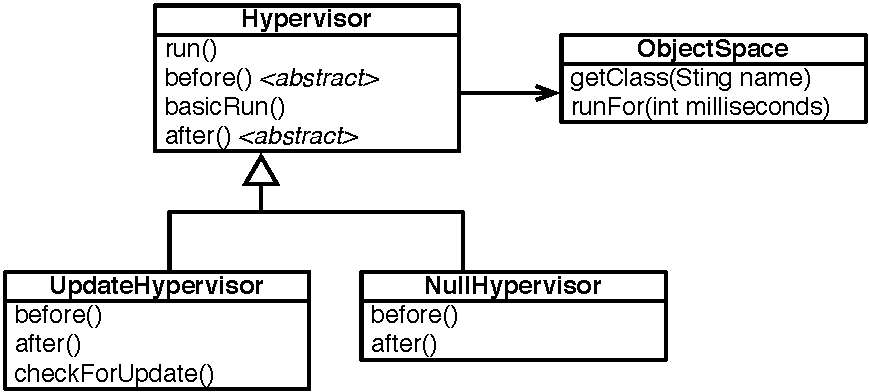
\includegraphics[width=.9\linewidth]{hypervisors}
\caption{\textbf{First-class Hypervisors.} .\label{fig:hypervisors}}
\end{figure}

\begin{code}
Hypervisor>>run [
    self before.
    self basicRun.
    self after.
]

Hypervisor>>basicRun [
    objectSpace runFor: 200.
]

UpdateHypervisor>>before [
    self checkForUpdate.
]

UpdateHypervisor>>checkForUpdate [
    "We check if a given file exists"
    'update.txt' asFile exists.
    ...
]
\end{code}

\section{Communication and Isolation} \label{sec:communication}\label{sec:isolation}

\gp{rewrite: cross message sends, literal translation, and boundary checks}

As explained in Section \ref{sec:isolation}, an objectspace is an isolated object graph in the sense that from the guest image there is no way to reach host objects. However, the opposite relation is possible: the host can manipulate completely the \objectspace.

The communication mechanism between host and guest images is based on the \emph{injection of objects} into the \objectspace. The host may install from simple literal objects such as strings or numbers, up to more complex objects like classes, methods. An \objectspace permits to \emph{send messages to objects} inside itself by injecting process with the specified code. Injected processes may have any arbitrary expression. The membrane objects can retrieve the result from the process' context once the execution is finished.

The \objectspace membrane ensures that object injection honors the transitive closure property. On one side, literal objects from the host are automatically translated to their representation in the \objectspace. An \objectspace implements the operations to transform literal objects (numbers, strings, symbols, some arrays and byte arrays) \emph{from and to} its internal representation.

On the other side, non literal objects are actually not created in the host and injected in the \objectspace. Non literal objects are directly created in the \objectspace, so the task of injecting the new object inside a graph is safe.

\gp{example!}


Note from the signatures presented that all mirror operations will return a mirror in exchange, and so, interaction with other objects inside the object space is mediated by Oz. Mirrors could give and revoke permissions on the wrapped object and enforce invariants to keep the model consistent~\cite{Teru13a}.
Oz provides also specific kinds of mirrors with high level APIs to manipulate objects with a specific format and/or behavior such as classes, methods, activation records or processes. We do not cover high level mirrors in this paper because they are not relevant to the bootstrap process.

\gp{next is old, see how to merge}

The manipulation of objects inside the \objectspace image cannot be achieved with a traditional message send mechanism. In the normal case, when a message send is performed, the virtual machine takes the selector symbol of the message and lookups in the class hierarchy method dictionaries of the receiver until it finds a method with the \emph{same}~(identical) selector. In our scenario, both host and guest images contain their own \ct{Symbol} class and symbol table. Then, when performing a \emph{cross image-message send} the method lookup mechanism takes a selector symbol from the host, lookups into the guest receiver's hierarchy, and finally fails because  the selector in the guest is (while maybe equals) not identical to the selector in the host. Also, forcing a \emph{cross image-message send} by using a guest's selector can leak host references to the guest: activating a guest method from the host gives the guest complete access to the host through the \ct{thisContext} special variable which reifies the stack on-demand.

To encapsulate and control the basic object manipulation, the object space fa\c{c}ade object provides mirrors~\cite{Brac04b}. Mirrors hide the internal representation of the objects inside the objectspace and expose reflective behavior. The guest is not aware of the existence of these mirrors.

All objects inside an \objectspace and reachable by reference can be retrieved by host's objects through the \objectspace facade and mirrors. 
There is no limitation nor restriction for object access. 
The host manipulates all objects in a homogeneous way through their mirrors. 

Additionally, specific mirrors are provided to manipulate objects with a specific format and/or behavior such as \ct{Class}, \ct{Metaclass}, \ct{MethodDictionary}, \ct{CompiledMethod}, \ct{MethodContext}, and \ct{Process}.

\section{Managing Runtime Execution} \label{sec:execution}

An \objectspace's execution is fully controllable from the host. The host can introspect and modify an \objectspace processes via mirrors to obtain information such as the method currently on execution, the values on the stack or the current program counter. Besides from those reflective operations, an \objectspace provides also operations to suspend, resume or terminate existing processes, and to install new ones.

\subsection{Direct VM Execution: Controlled cycles}

Pharo applications can be virtualized transparently, as no changes are required on them. They are, however, interrupted periodically in safe control points in which the hypervisor can check if an update is eventually necessary. A first-class hypervisor object allows us to have a flexible update mechanism: we can dynamically change it and easily prototype them.

To allow the hypervisor to control the virtualized runtime, we split the virtualized runtime execution in cycles. During each execution cycle, the virtualized runtime runs unmanaged using the full capacity of the VM. When the cycle finishes the virtualized runtime is suspended in the next suspension point if finds, and the control is returned to the hypervisor runtime. The hypervisor runtime will act~(check if there are pending updates, install updates or nothing) and then resume the execution of the application from the last suspension point.

Our implementation presents an execution cycle of 200ms that allows us to have fine grained control while the virtualized application has still place to run. We use as suspension points backjumps found in the executed bytecode and message sends. In such a way, we ensure that the execution stack is in a consistent state after it is interrupted.

\begin{figure}[ht]
\center
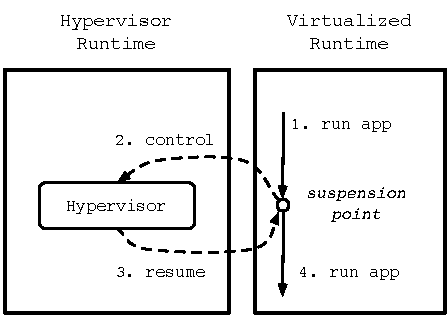
\includegraphics[width=.6\linewidth]{execution_cycle}
\caption{\textbf{Execution Cycle.} \label{fig:execution_cycle}}
\end{figure}

The \objectspace provides fine-grained control on the guest execution. An \objectspace controls the amount of CPU used by the guest image. \sd{can you do that for real? CPU control?}\gp{We can give an objectspace a window of 20ms to run and then we get back control so It's our decision if we give it 20 more or not :)}This way, a virtual image can be customized for scenarios like for example testing, CPU usage analysis, or old hardware simulation. For example, it may restrict its processes to run during only 300 milliseconds every second for either.

\begin{description}
\item[Code execution.] Oz provides with operations to manipulate the processes/threads of the guest language kernel. In particular, the \ct{runForTime()} operation will execute the guest language kernel with whichever processes it has installed, directly on the VM.
\begin{code}
List<mirror> getProcesses();
mirror createProcessDoing(String expression);
void runForTime(int milliseconds);
\end{code}
%\caption{\textbf{Code of the Builder implementing the same logic as in \ct{Dictionary>>initialize}.}\label{code:logic_dup2}}
%\end{figure}
\end{description}

The language primitives are those operations that the VM exposes to the language. The interpreter uses this interface to execute primitive operations that appear in the language definition.

\begin{code}
objectSpace\{
    /* For bootstrapping purposes when no class is available */
    mirror executePrimitive(primitiveID aPrimitive, Array args); 
\}
\end{code}



\subsection{Simulated Execution: AST interpretation}

The bootstrapping interpreter is a code interpreter, potentially written in language different from the bootstrapped one, that interprets code expressed in the bootstrapped language. Its design present the following important points that allow it to execute code inside the language kernel before it reaches the execution point:

\begin{description}
\item[Alternative method lookup.] Before reaching the execution point, the class hierarchy of the language kernel is incomplete, or part of its methods is not yet installed. An alternative method lookup mechanism is put in place in the bootstrapping interpreter to allow message sending before we reach the execution point: methods are looked up in the definition of the language instead of the hierarchy in the language kernel; a mapping is kept between classes created in the language kernel and their definitions in the language definition to know where the lookup should start.

\item[Automatic class stubs.] The bootstrapping interpreter does also solve most of the well known bootstrapping issues~(\eg how to create a class before a class exists) in a generic way by using class stubs. When an inexistent class is needed during the bootstrap process, the interpreter creates an empty class to take it place respecting the VM format for it. The interpreter will be able to create instances of this class and map it to its corresponding definition to perform the method lookup. This class cannot, however, initially perform reflective operations as it does not contain any reflective information. When the real class is created later on in the process, it replaces the stub.
\end{description}

\section{Virtualization Overhead Benchmarks} \label{sec:virtualization_benchmarks}

We benchmarked our prototype implementation using a subset of the computer language benchmarks game\footnote{\url{http://benchmarksgame.alioth.debian.org/}}. We executed our benchmarks in four different setups, in Table \ref{tb:benchmarks}. We first benchmarked the Vanilla Pharo VM without any of our changes, to make it our base of comparison. Afterwards, we benchmarked our solution in three different setups:

\begin{description}
\item[Null Hypervisor.] A hypervisor performing no particular action.
\item[File Checking Hypervisor.] A hypervisor checking the existence of a File on each monitoring cycle.
\item[Stack Checking Hypervisor.] A hypervisor checking the execution stack of the target application on each monitoring cycle. This benchmark forces in our implementation a reification of the execution contexts~(stack frames).
\end{description}

\begin{landscape}
 \begin{table*}[p]
 \small
 	\centering
 	\begin{tabular}{|l|c|c|c|c|}
			\hline
			\textbf{Benchmark}
 			& \textbf{Vanilla VM (1x)}
			& \textbf{Null Hypervisor}
			& \textbf{File Checking Hypervisor}
			& \textbf{Stack Checking Hypervisor}\\
		\hline
		RegexDNA & 5711ms +/-22 & 5878ms +/-18 & 6142ms +/-11 & 6555ms +/-424 \\\hline
		KNucleotide & 94.00ms +/-0.85 & 100.1ms +/-3.4 & 105.8ms +/-3.2 & 134.4ms +/-3.7 \\\hline
		SpectralNorm & 79.8ms +/-1.4 & 86.6ms +/-1.4 & 92.7ms +/-6.0 & 110.7ms +/-1.7 \\\hline
		BinaryTrees & 36.80ms +/-0.65 & 37.10ms +/-0.83 & 35.30ms +/-0.66 & 65.20ms +/-0.93 \\\hline
		Mandelbrot & 422.3ms +/-1.4 & 488.0ms +/-6.5 & 494.9ms +/-3.4 & 632ms +/-23 \\\hline
		ReverseComplement & 5.40ms +/-0.48 & 6.80ms +/-0.24 & 6.80ms +/-0.59 & 8.00ms +/-0.60 \\\hline
		ThreadRing & 2.50ms +/-0.41 & 2.50ms +/-0.56 & 2.70ms +/-0.90 & 3.20ms +/-0.80 \\\hline
		PiDigits & 0.90ms +/-0.69 & 0.70ms +/-0.66 & 0.70ms +/-0.66 & 0.90ms +/-0.69 \\\hline
		Meteor & 2260.2ms +/-2.6 & 2398.2ms +/-8.5 & 2479ms +/-16 & 3677ms +/-267 \\\hline
		NBody & 21.10ms +/-0.57 & 21.70ms +/-0.66 & 22.6ms +/-1.4 & 37.7ms +/-1.5 \\\hline
%		FannkuchRedux & 0.00ms +/-0.00 & 0.00ms +/-0.00 & 0.20ms +/-0.36 & 0.00ms +/-0.00 \\\hline
		Fasta & 4.30ms +/-0.54 & 5.20ms +/-0.65 & 5.70ms +/-0.61 & 9.30ms +/-0.39 \\\hline
 	\end{tabular}
	\vspace*{0.2cm}
 	\caption{\small\textbf{Language Virtualization Overhead.} Comparing the startup time of a ruby application with the same in Pharo or Candle using a snapshot.\label{tb:benchmarks}}
 \end{table*}
\end{landscape}
% =============================================================================
\input{chapter-footer.tex}